%!TEX root = ./provabeamer.tex


\section{Background}

%Gaussian graphical models-------------------------------
\subsection{Gaussian Graphical Models}
\begin{frame}{Gaussian Graphical Models}

    Models for the \alert{conditional dependence structure} among variables, represented through an undirected graph $G=(V,E)$
    \begin{align*}
    \bm{x}_{1}, \ldots, \bm{x}_{n} \mid \bm{K} &\iid N_{p}(\bm{0},\bm{K}^{-1}), \bm{K}=\Sigma^{-1}, \bm{K} \in \mathbb{R}^{p\times p}  %%%%add bold
    \end{align*}
Conditional independence described through a \alert{map} between a \alert{graph} and a family of multivariate \alert{probability models}
\begin{align*}
Y_{i}\indep Y_{j} \mid Y_{-(ij)} \iff (i,j) \notin E \iff k_{ij}=0
\end{align*}
Usual prior for $\bm{K}$ conditionally to the graph is a G-Wishart
\begin{align*}
    \bm{K} \mid G &\iid \GWish(B,d)
\end{align*}
$G$ is a r.v. in the space of undirected graphs with $p$ nodes.\\
If we assume a possible \alert{grouping} of the variables, we need a prior $\pi(G)$ that induces a \alert{block structure on its adjacency matrix}.
\end{frame}


%%TO DO @Teo 
%Add bold sigma
%Add the image - STAVO PENSANDO, MA SE NE METTESSIMO DUE? UNA CON UN GRAFO CON ELEMENTI DA 1 A P STRUTTURA E UNA TABELLA - OK CHE E' SIMILE A QUELLO DI COLOMBI BUT STILL
%%

 

%Stochastic Block Models -----------------------
\subsection{Stochastic Block Models}
\begin{frame}{Stochastic Block Models for the prior on $G$}

Given a random network of data, SBM \alert{infere a node partition} based on similarity of connectivity patterns. Let
\begin{itemize}
    \item $H$ be the fixed number of clusters
    \item $\bm{z} \in \mathbb{R}^p$ be the vector of group memberships, $z_{i} \in \{1,\ldots,H\}$
\end{itemize} 

Then the model for the prior of $G$ conditionally on $\bm{z}$ is the following
\begin{align*}
    G_{ij} \mid \bm{z} &\ind\  f_{G}(G \mid \bm{z}) , \quad 1 \le i < j \le p \\ %alternativr G_{ij} \in {Edges}
    \bm{z} &\iid\ f_{z}(\bm{z})
\end{align*}
Where $f_{G}(G \mid \bm{z})$ and $f_{z}(\bm{z})$ can be chosen from different parametric families
\pause
\begin{center}
    Critical task: \alert{identification of the number of clusters $H$}
\end{center}

\end{frame}







\begin{frame}{Choosing the number of clusters $H$}

$H$ is usually estimated \alert{before} running the model. However
\begin{itemize}
    \item uncertainty at this stage is ignored (\alert{error quantification})
    \item the model does not account for new clusters (\alert{prediction})
\end{itemize}
\vspace*{0.5cm}
\pause
\alert{Extended stochastic block models (ESBM)}\\
Use priors for $\bm{z}$ that naturally allow to adaptively modify the number of groups $H$, \emph{e.g.},
\begin{itemize}
    \item Finite Dirichlet
    \item Infinite Dirichlet
    \item Mixture of Finite Mixtures
\end{itemize}

\pause
\begin{center}
    \alert{Most of the ESBM models do not pose constraints\\
    on the ordering of the nodes when generating the partition,\\
    that may be of relevance in real-life context (i.e., gene expression).}    
\end{center}


\end{frame}








%Changepoint models------------------
\subsection{Changepoint Models}
\begin{frame}{Changepoint Models}
    %\fg{0.4}{changepoint}
    Consider a process where at certain \alert{changepoints} the underlying generating mechanism changes. Let $\bm{x}=(x_{1},\ldots,x_{n})$ be \alert{ordered} observations each depending on a $\vartheta_{i}.$
    \[
        f(x_{1},\ldots,x_{n} \mid \vartheta_1, \vartheta_2, \ldots, \vartheta_{k+1}, \bm{z})=\prod_{j=1}^{k+1} \prod_{i=\tau_{j-1}+1}^{\tau_j} f(x_i \mid \vartheta_j)
    \]
    where $\tau_j$ are changepoint times and $z_{i} = 1$ if it's a changepoint, $0$ otherwise.
    We borrow the concept of \alert{generating a random partition with ordering constraints}:\footnote{$\vartheta$ can be marginalized out.}
    \begin{align*}
        \pi(\bm{z}, \bm{\vartheta} \mid \bm{y}) & \propto f(\bm{y} \mid \bm{\vartheta}, \bm{z}) \pi(\bm{\vartheta} \mid \bm{z}) \pi(\bm{z}) \\
        &=\left(\prod_{j=1}^{k+1} \prod_{i=\tau_{j-1}+1}^{\tau_j} f(y_i \mid \vartheta_j)\right)\left(\prod_{j=1}^{k+1} \pi(\vartheta_j)\right) \pi(\bm{z})
    \end{align*}
\end{frame}








%----------------------------------------
% Project goals
%-------------------------------------
\section{Project goals and next steps}


\begin{frame}{Goal of the project and next steps}

\alert{Goal}

Propose a \alert{new prior} that accounts for
%a random partition of the nodes, respects their ordering constraints and allows to learn a block structured graph
\begin{itemize}
    \item Ordering Constraint: taking advantage of the study of changepoint models
    %\item Random partition: using nonparametric prior on ordered partitions
    \item Block Structure: using a stochastic block model prior
\end{itemize}
\vspace*{0.5cm}
\pause
\alert{Next steps}
\begin{itemize}
    \item understanding and implementing the sampling strategy;
    \item using a nonparametric prior on ordered partitions.
\end{itemize}

\end{frame}

\begin{frame}{Main references}
    % GGM
    \nocite{colombiLearningBlockStructured2022a}
    \nocite{mohammadiBayesianStructureLearning2015a}
    % SBM
    \nocite{legramantiExtendedStochasticBlock2022}
    % Changepoint
    \nocite{bensonAdaptiveMCMCMultiple2018}
    \nocite{martinezNonparametricChangePoint2014}
    
    
    %biblatex
    %\printbibliograph
    %\renewcommand*{\bibfont}{\small}
    %bibtex
    \bibliographystyle{plain} % We choose the "plain" reference style
    \bibliography{bibliography} % Entries are in the refs.bib file
\end{frame}

\begin{frame}[plain]
    % Add background to content page
    \AddToShipoutPictureFG*{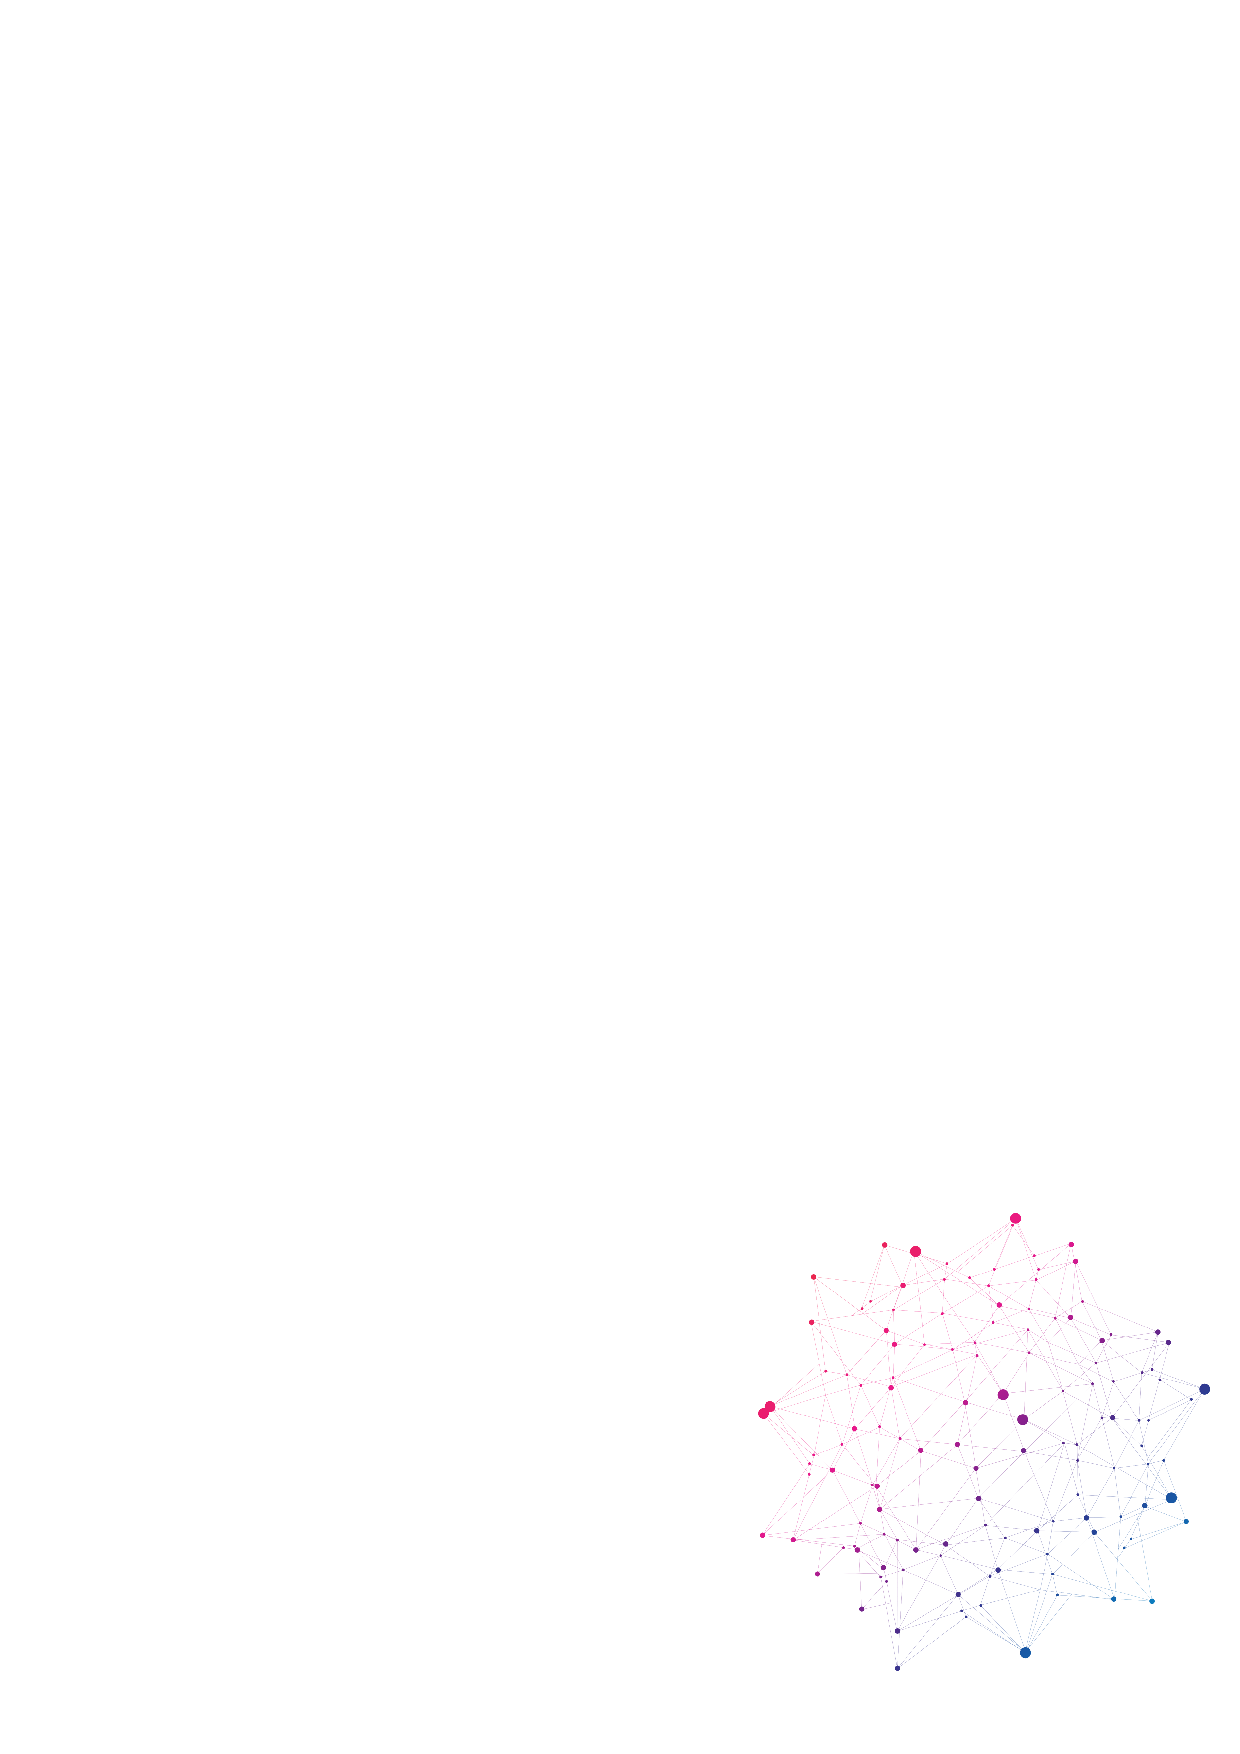
\includegraphics[width=\paperwidth]{Images/background.pdf}}
    \vspace*{1.2cm}
    \hspace*{1cm}{\Large Thank you!}\\
    \vspace*{0.6cm}
    \pause
    \hspace*{1cm}{\Huge \alert{Any questions?}}
\end{frame}


















%tenere?
\section*{Extra}
%Stochastic Block Models -----------------------
\begin{frame}{Stochastic Block Models for the prior on G}

\begin{align*}
    G_{ij} \mid \Theta,\bm{z} &\iid \Be(\theta_{ij}),  G \in \mathbb{R}^{p \times p}, \quad \theta_{ij} = \Theta_{z_{i}z_{j}}, \quad 1 \le i < j \le p \\ 
    \Theta_{z_{i}z_{j}} &\iid \Beta(\alpha, \beta)\\
    \bm{z} &\iid \pi_{z}(\bm{z}), \quad \bm{z} \in \mathbb{R}^p
\end{align*}
$\Theta$ can be marginalized out via beta-binomial conjugacy.
%Tattica: farei comparire la figura con un tap, e intanto si commenta che "per brevità non entriamo nel dettaglio ma se sono interessati si"
\fg{0.9}{sbm}
%Aggiungere da dove viene la caption
 %% Critical task: \alert{identification of the number of clusters H}
{\scriptsize From ``Colombi et al. Learning block structured graphs in Gaussian graphical models.''}
\end{frame}


